%%%%%%%%%%% Exposición 03
\subsection[Expositor: Zayra Paulina Galván Ordoñez.]{Segmentos de líneas punzantes.}
\textbf{Obejetivo:} Algoritmo para determinar las líneas que interseca a cada uno de
los $n$ segmentos de línea dados en el plano.\newline

\textbf{Desarrollo:} Para un conjunto $S$ de $n$ segmentos de línea en el plano. Si queremos calcular
todas las líneas punzantes, entonces analicemos dos posibles casos:
\begin{enumerate}
\item Si sólo hay un segmento de línea en el conjunto $S$.
  Entonces, la región punzante es la doble cuña de este segmento.
  
  \begin{center}
    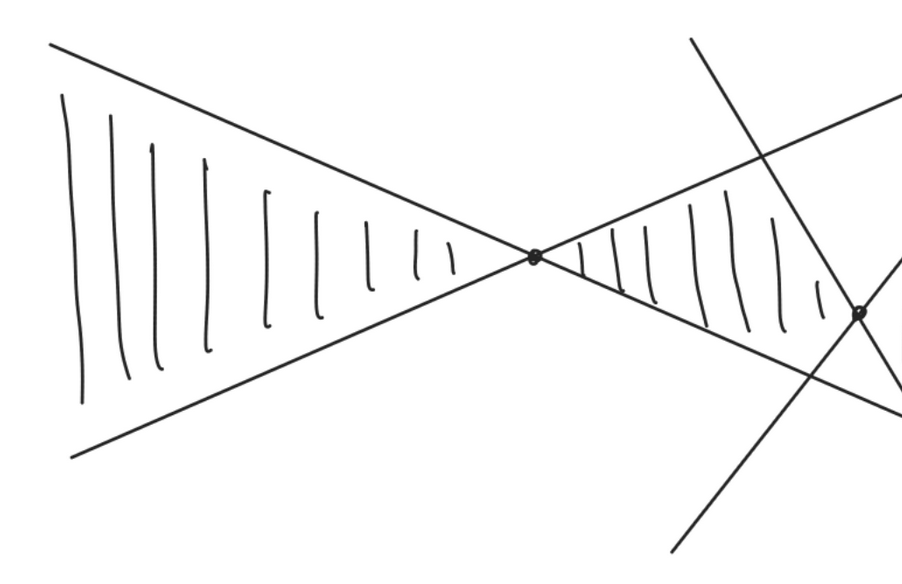
\includegraphics[scale=0.30]{./Im2.png}\\[0.4cm]
  \end{center}
\item Si hay al menos dos segmentos, dividir el conjunto $S$ en dos subconjuntos
  de igual tamaño y calcular la región punzante de ambos subconjuntos de manera
  recursiva. La región punzante de todo el conjunto es la intersección de las
  regiones punzantes de los subconjuntos.
\end{enumerate}
